\documentclass[11pt]{article}
\usepackage[final]{graphicx}
\usepackage{subcaption}
\usepackage[utf8]{inputenc}
\usepackage{listings}
\usepackage{color}
\usepackage{fancyhdr}
\usepackage{enumerate}
\usepackage{enumitem}
\usepackage{hyperref}
\usepackage{wordlike}

% \makeatletter
% \setlength{\@fptop}{0pt}
% \makeatother

% Make hyperlinks prettier
\hypersetup{
    colorlinks=true,
    linkcolor=blue,
    filecolor=magenta,      
    urlcolor=cyan,
}

% Python code formatting
\definecolor{codegreen}{rgb}{0,0.6,0}
\definecolor{codegray}{rgb}{0.5,0.5,0.5}
\definecolor{codepurple}{rgb}{0.58,0,0.82}
\definecolor{backcolour}{rgb}{0.95,0.95,0.92}
 
\lstdefinestyle{mystyle}{
    backgroundcolor=\color{backcolour},
    commentstyle=\color{codegreen},
    keywordstyle=\color{magenta},
    numberstyle=\tiny\color{codegray},
    stringstyle=\color{codepurple},
    basicstyle=\small,
    breakatwhitespace=false,
    breaklines=true,
    captionpos=t,
    keepspaces=true,
    numbers=left,
    numbersep=5pt,
    showspaces=false,
    showstringspaces=false,
    showtabs=false,
    tabsize=2
}

\lstset{style=mystyle}

\setlist{parsep=0pt,listparindent=\parindent}

% Header settings  
\pagestyle{fancy}
\fancyhf{}
\rhead{10/06/2016}
\chead{Paul Ruess}
\lhead{CE 385S -- Homework 3}
\rfoot{Page \thepage}

\begin{document}

\section*{\centerline{Homework 3 -- Problem 4}}

This project has been improved since the previous deliverable in the following ways: 

\begin{enumerate}
  \item Using the hydraulic properties computed with the Height Above Nearest Drainage (HAND) method, I have back-calculated the average manning's $n$ for each United States Geological Survey (USGS) rating curve in the Onion Creek, TX watershed. 
  \item For each USGS gage station, I have found the first instance of flow (ie. flow of 0.01 cfs) and mapped the associated stage-height as the channel bottom-depth. 
  \item Using the back-calculated manning's $n$, I have tilted the HAND rating curve for an approximate fit to the USGS rating curve with a new bottom-depth. 
\end{enumerate}

Examples of a few rating curves, as compared to their previously "manually" optimized manning's $n$ values, are included in figures 1, 2 and 3. Note that these graphs are not strictly comparable, due to the fact that changes have been made to both the USGS curve (bottom-depth shift) and the HAND curve (different manning's $n$ used). Furthermore, it is important to be aware that an average manning's $n$ (from the various manning's $n$ values calculated from the USGS data at each 1-foot interval) was applied to the HAND rating curve, and this averaging is likely not the best approach for this application; possible improvements could be made by using a root-mean-square-error approach for assessing the optimal manning's $n$ with this back-calculating approach. Finally, it is important to be aware that, though these automatic adjustments seem to fit the USGS rating curves fairly well, this will not be a sustainable model for large-scale rating curve optimization as it relies entirely on USGS rating curves for determining which manning's $n$ to use for the HAND rating curve snapping. 

% \begin{equation}
% Q = \frac{k}{n}AR^\frac{2}{3}S^\frac{1}{2}
% \end{equation}
% where: 
% \begin{description}
% \item[Q] is the discharge (L\textsuperscript{3}/T; ft/s, m/s);
% \item[A] is the cross-sectional area (L\textsuperscript{2}; ft\textsuperscript{2}, m\textsuperscript{2});
% \item[R] is the hydraulic radius (L; ft, m);
% \item[S] is the channel bed slope at constant water depth (L/L, ft/ft, m/m).
% \item[k] is a conversion factor, 1.0 for SI units and 1.49 for English units.
% \end{description}

% \vspace{1ex}
% \clearpage

\begin{figure}[b!]
\makebox[\linewidth][c]{
\begin{subfigure}{0.65\textwidth}
  \centering
  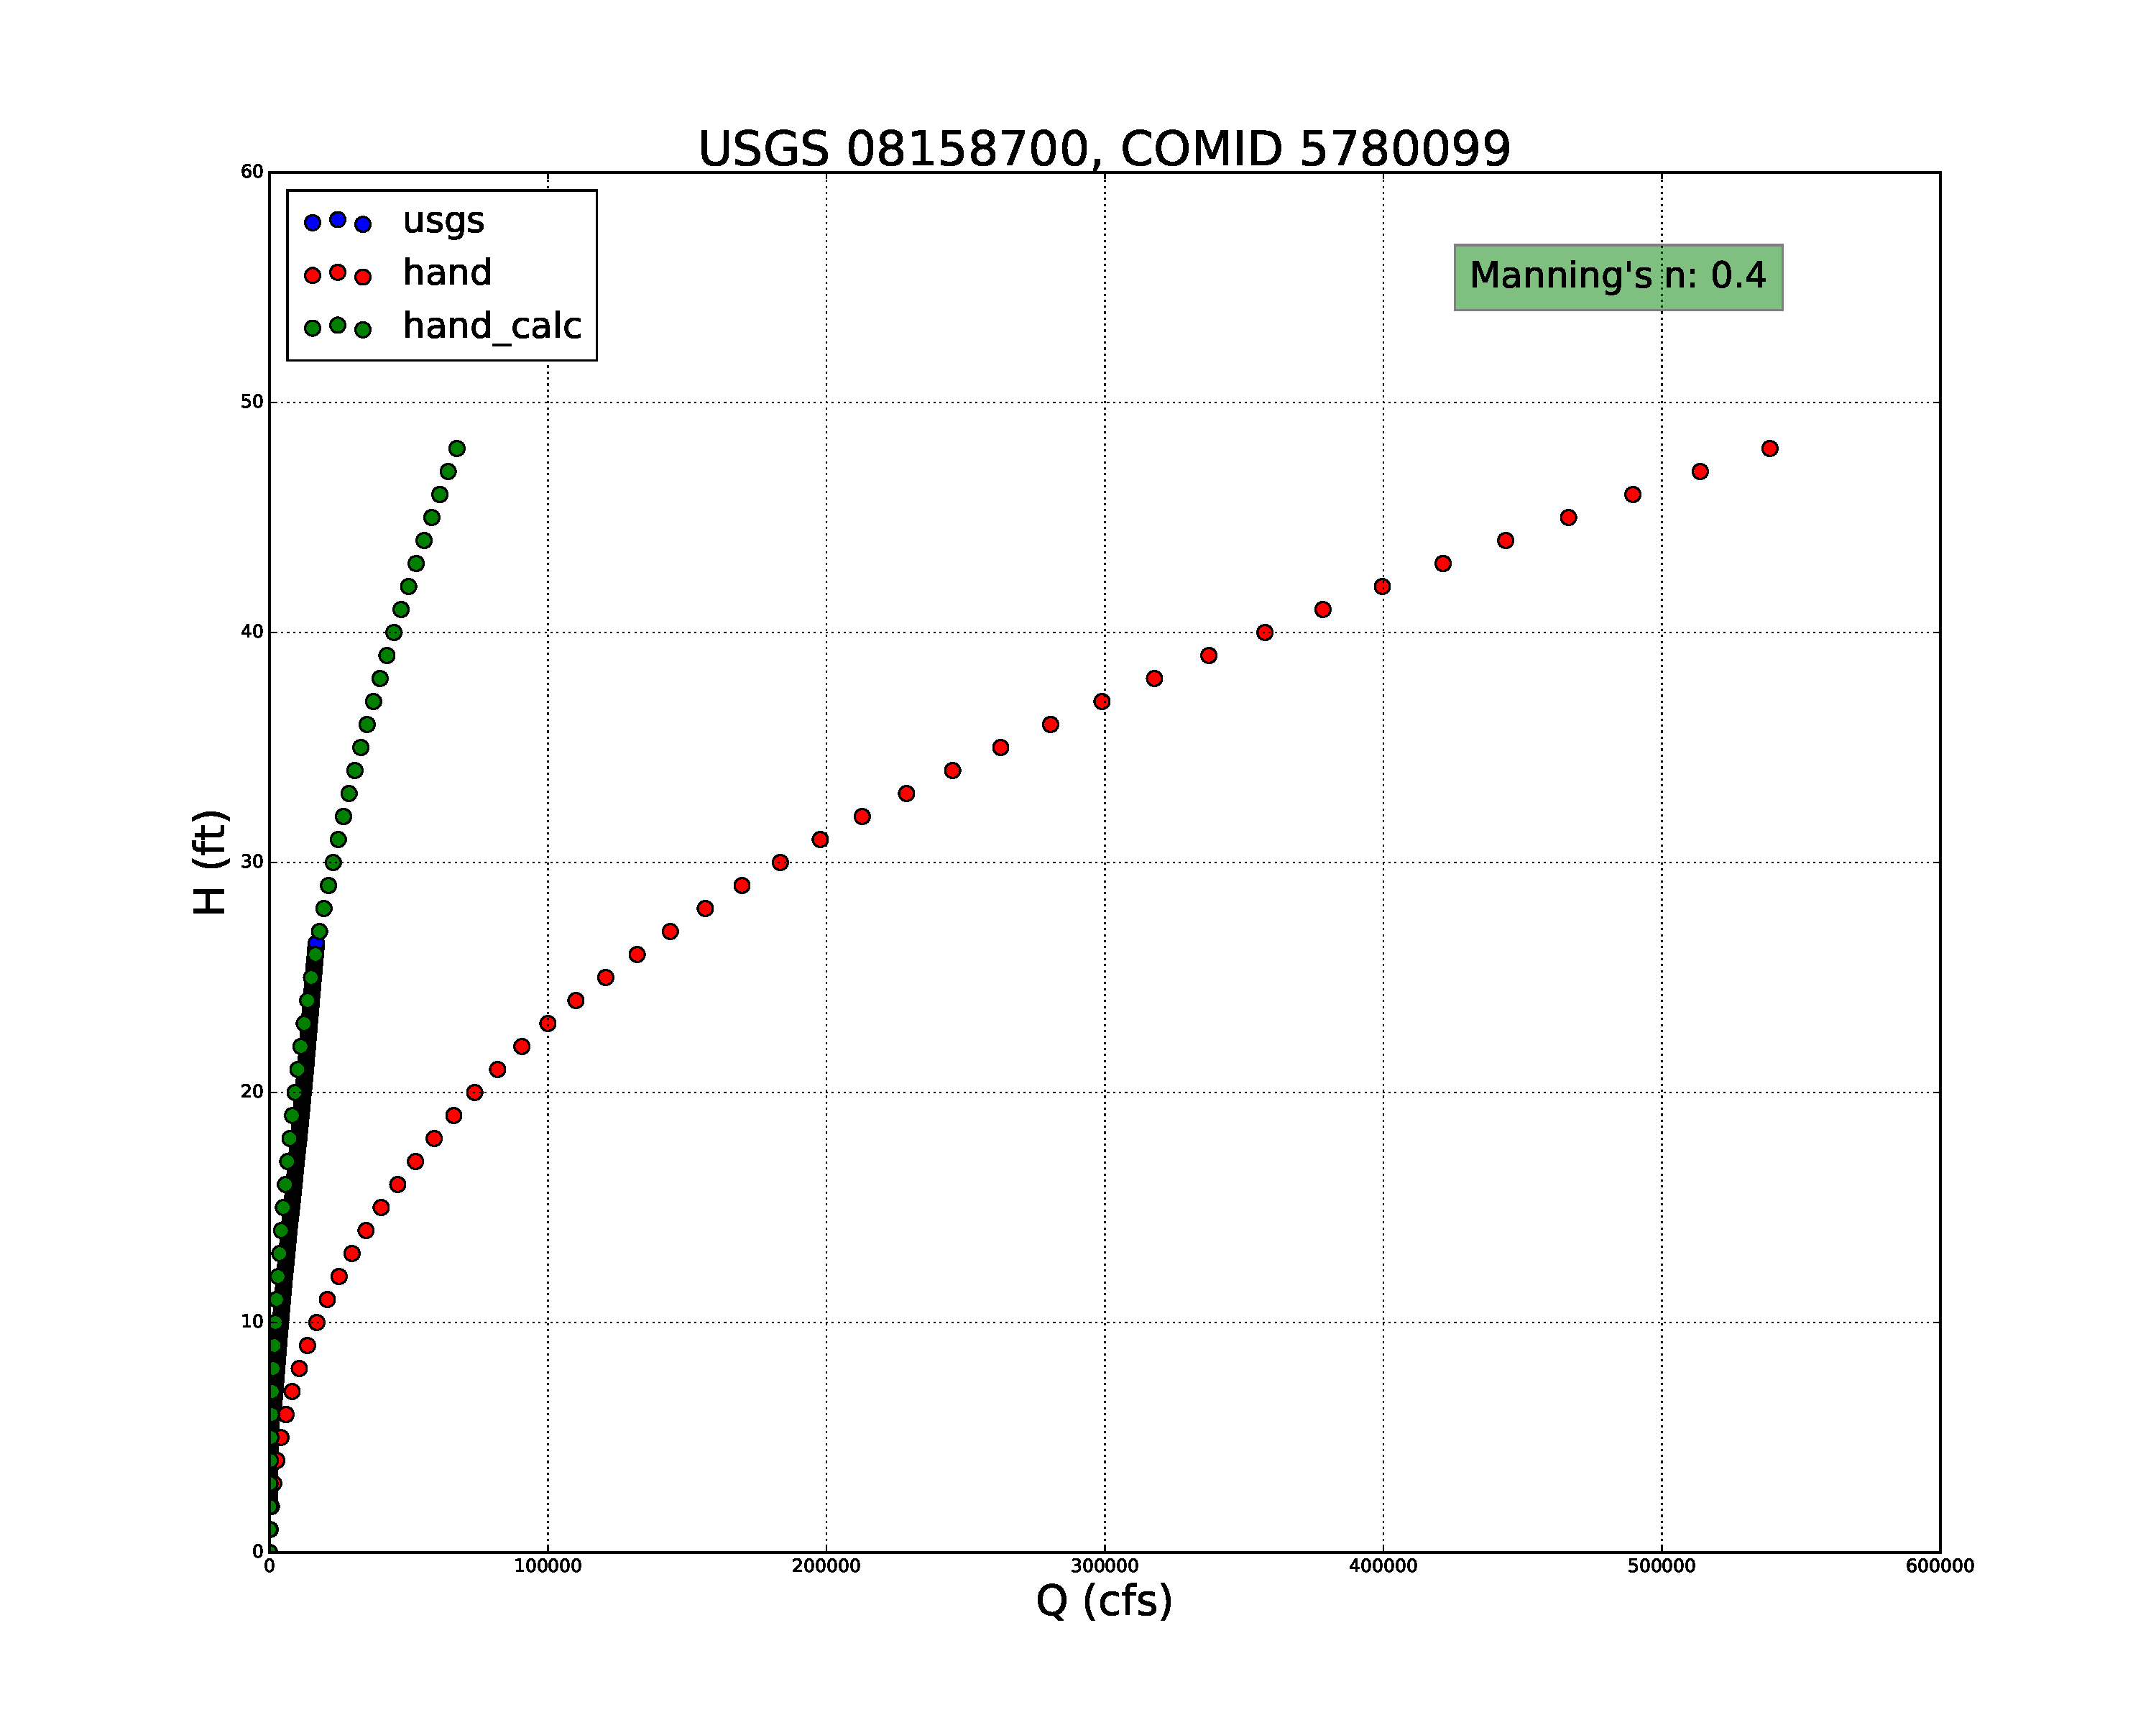
\includegraphics[width=\linewidth]{manualresults/rc_comid_5780099.pdf}
  \caption{Manually-Adjusted Rating Curve}\label{fig:a}
\end{subfigure}\hspace*{\fill}
\begin{subfigure}{0.65\textwidth}
  \centering
  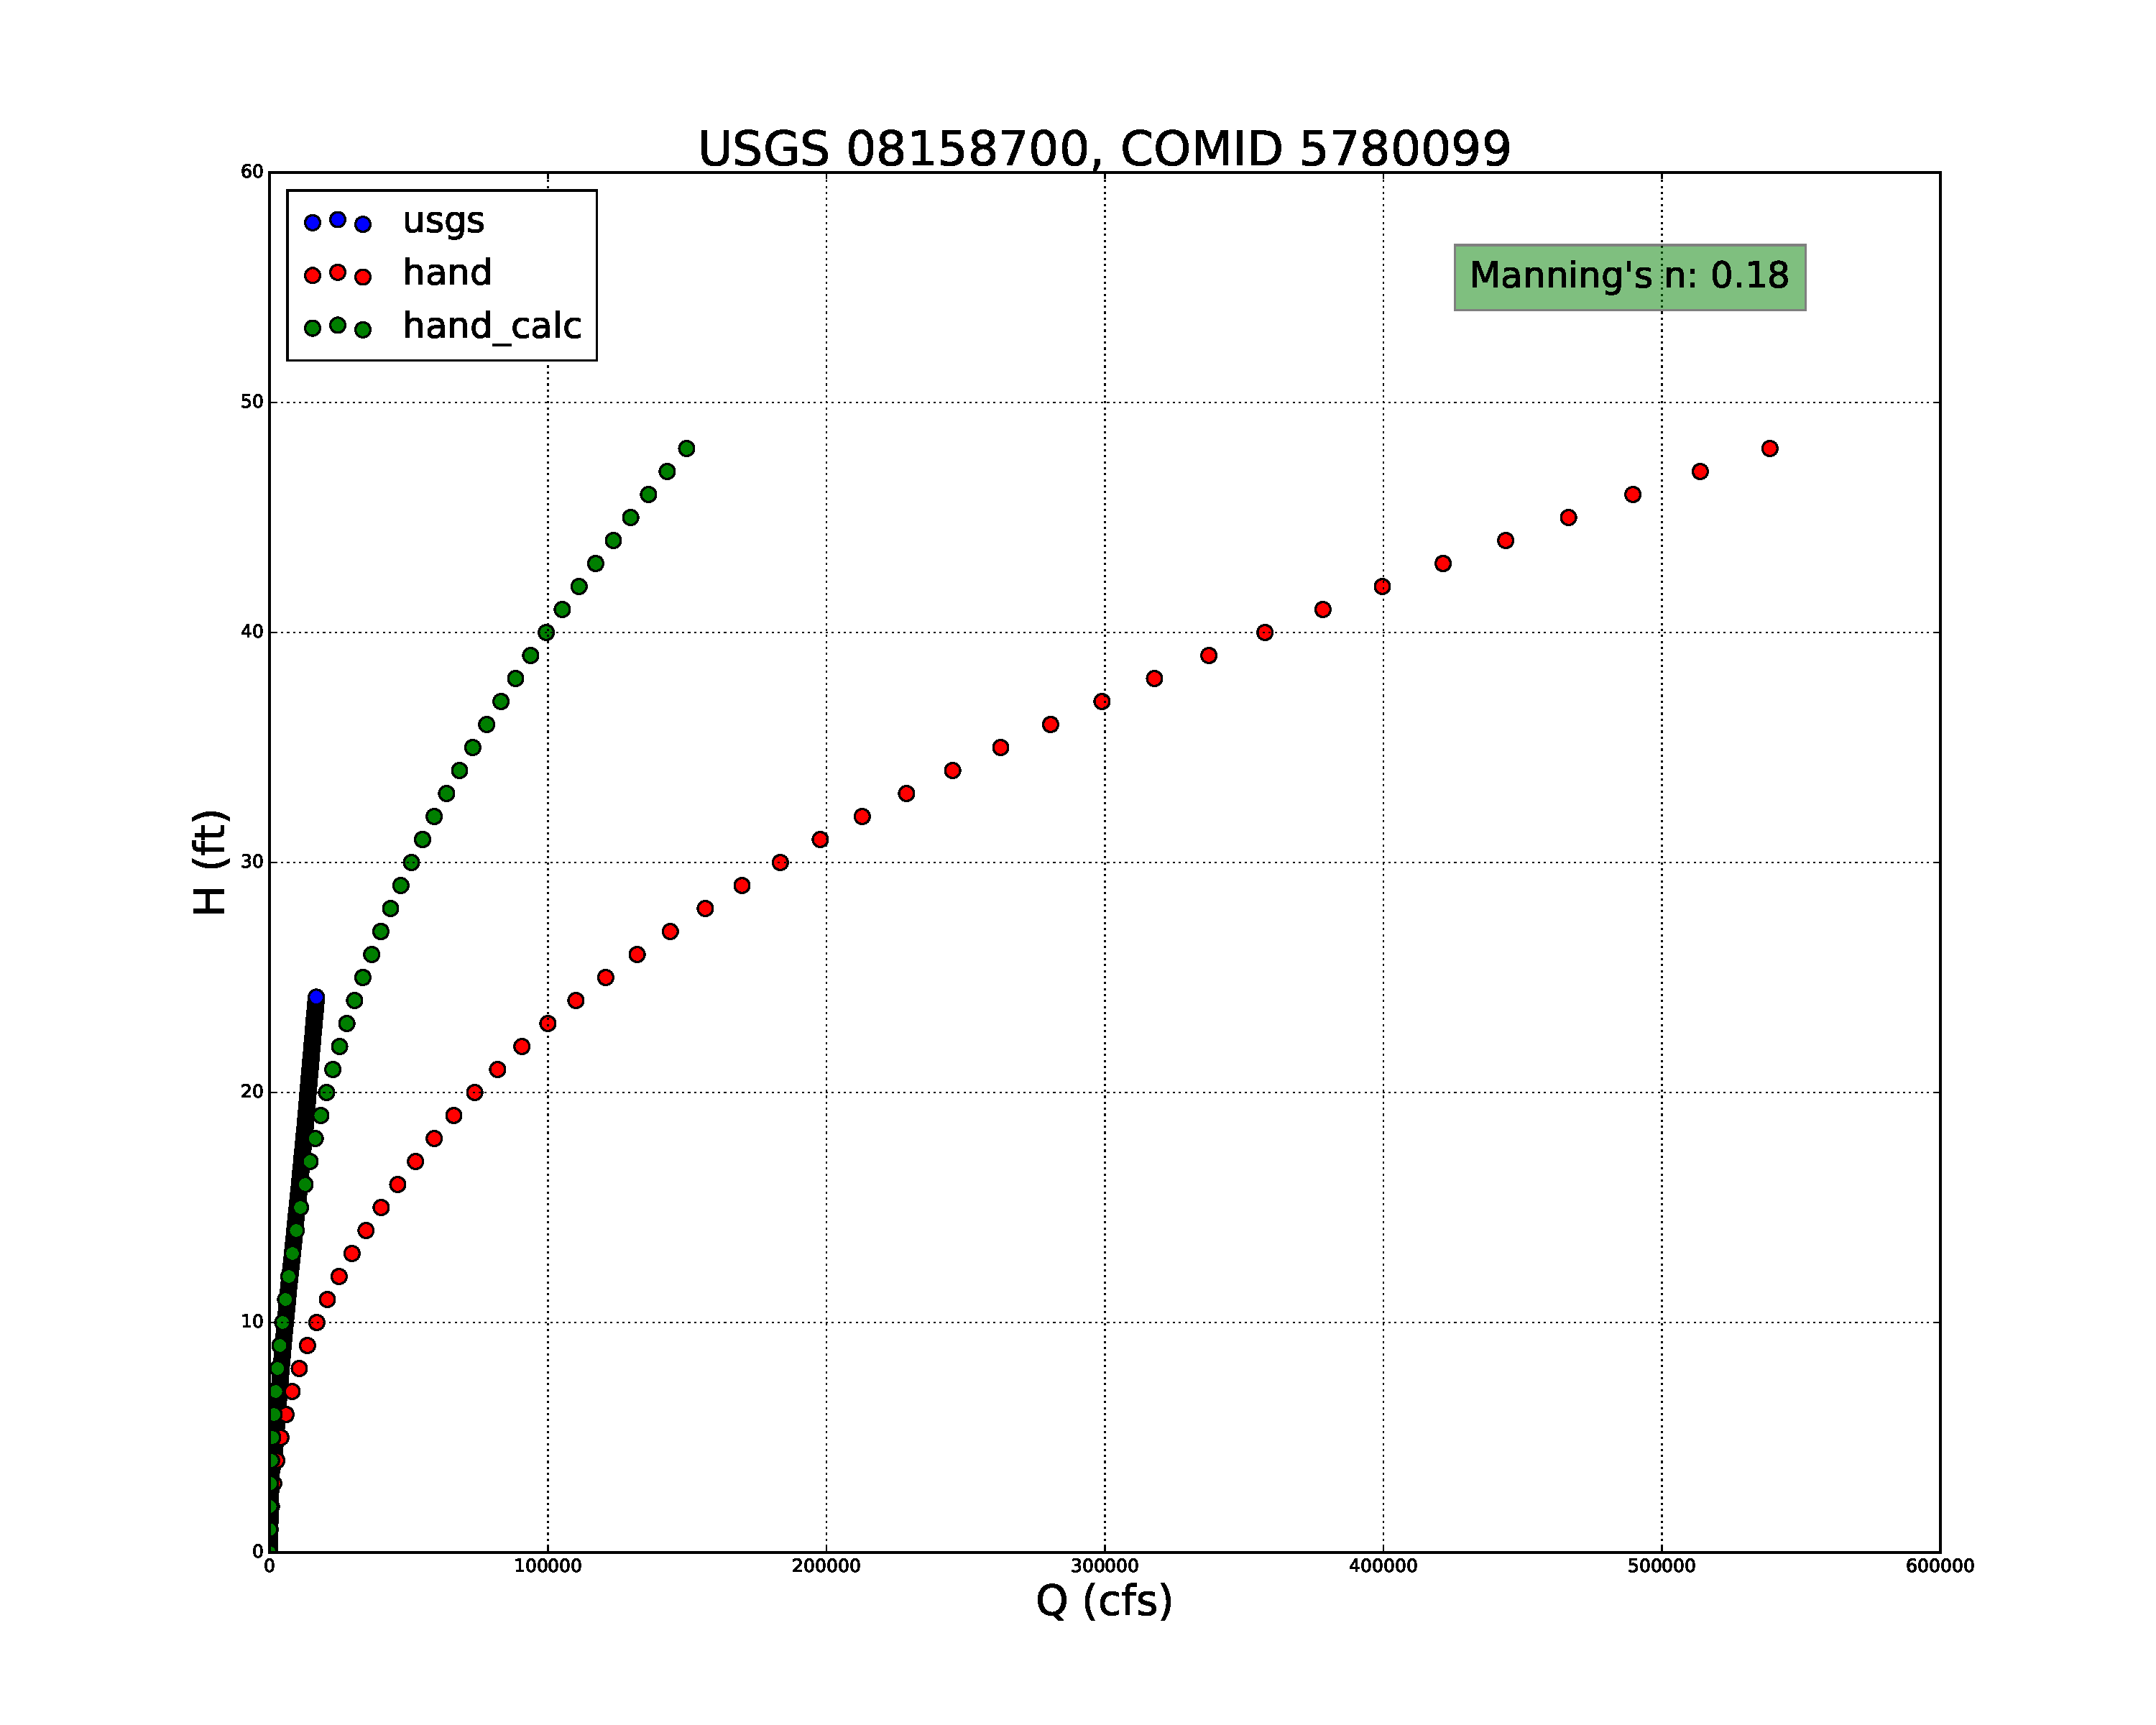
\includegraphics[width=\linewidth]{autoresults/rc_comid_5780099.pdf}
  \caption{Automatically-Adjusted Rating Curve}\label{fig:b}
\end{subfigure}\hspace*{\fill}
}
\caption{Manual vs. Automatic Adjustments for COMID 5780099 Rating Curve} \label{fig:2}
\end{figure}

% \begin{figure}[b!]
% % \ContinuedFloat
% % \smallskip
% \makebox[\linewidth][c]{
% \begin{subfigure}{0.65\textwidth}
%   \centering
%   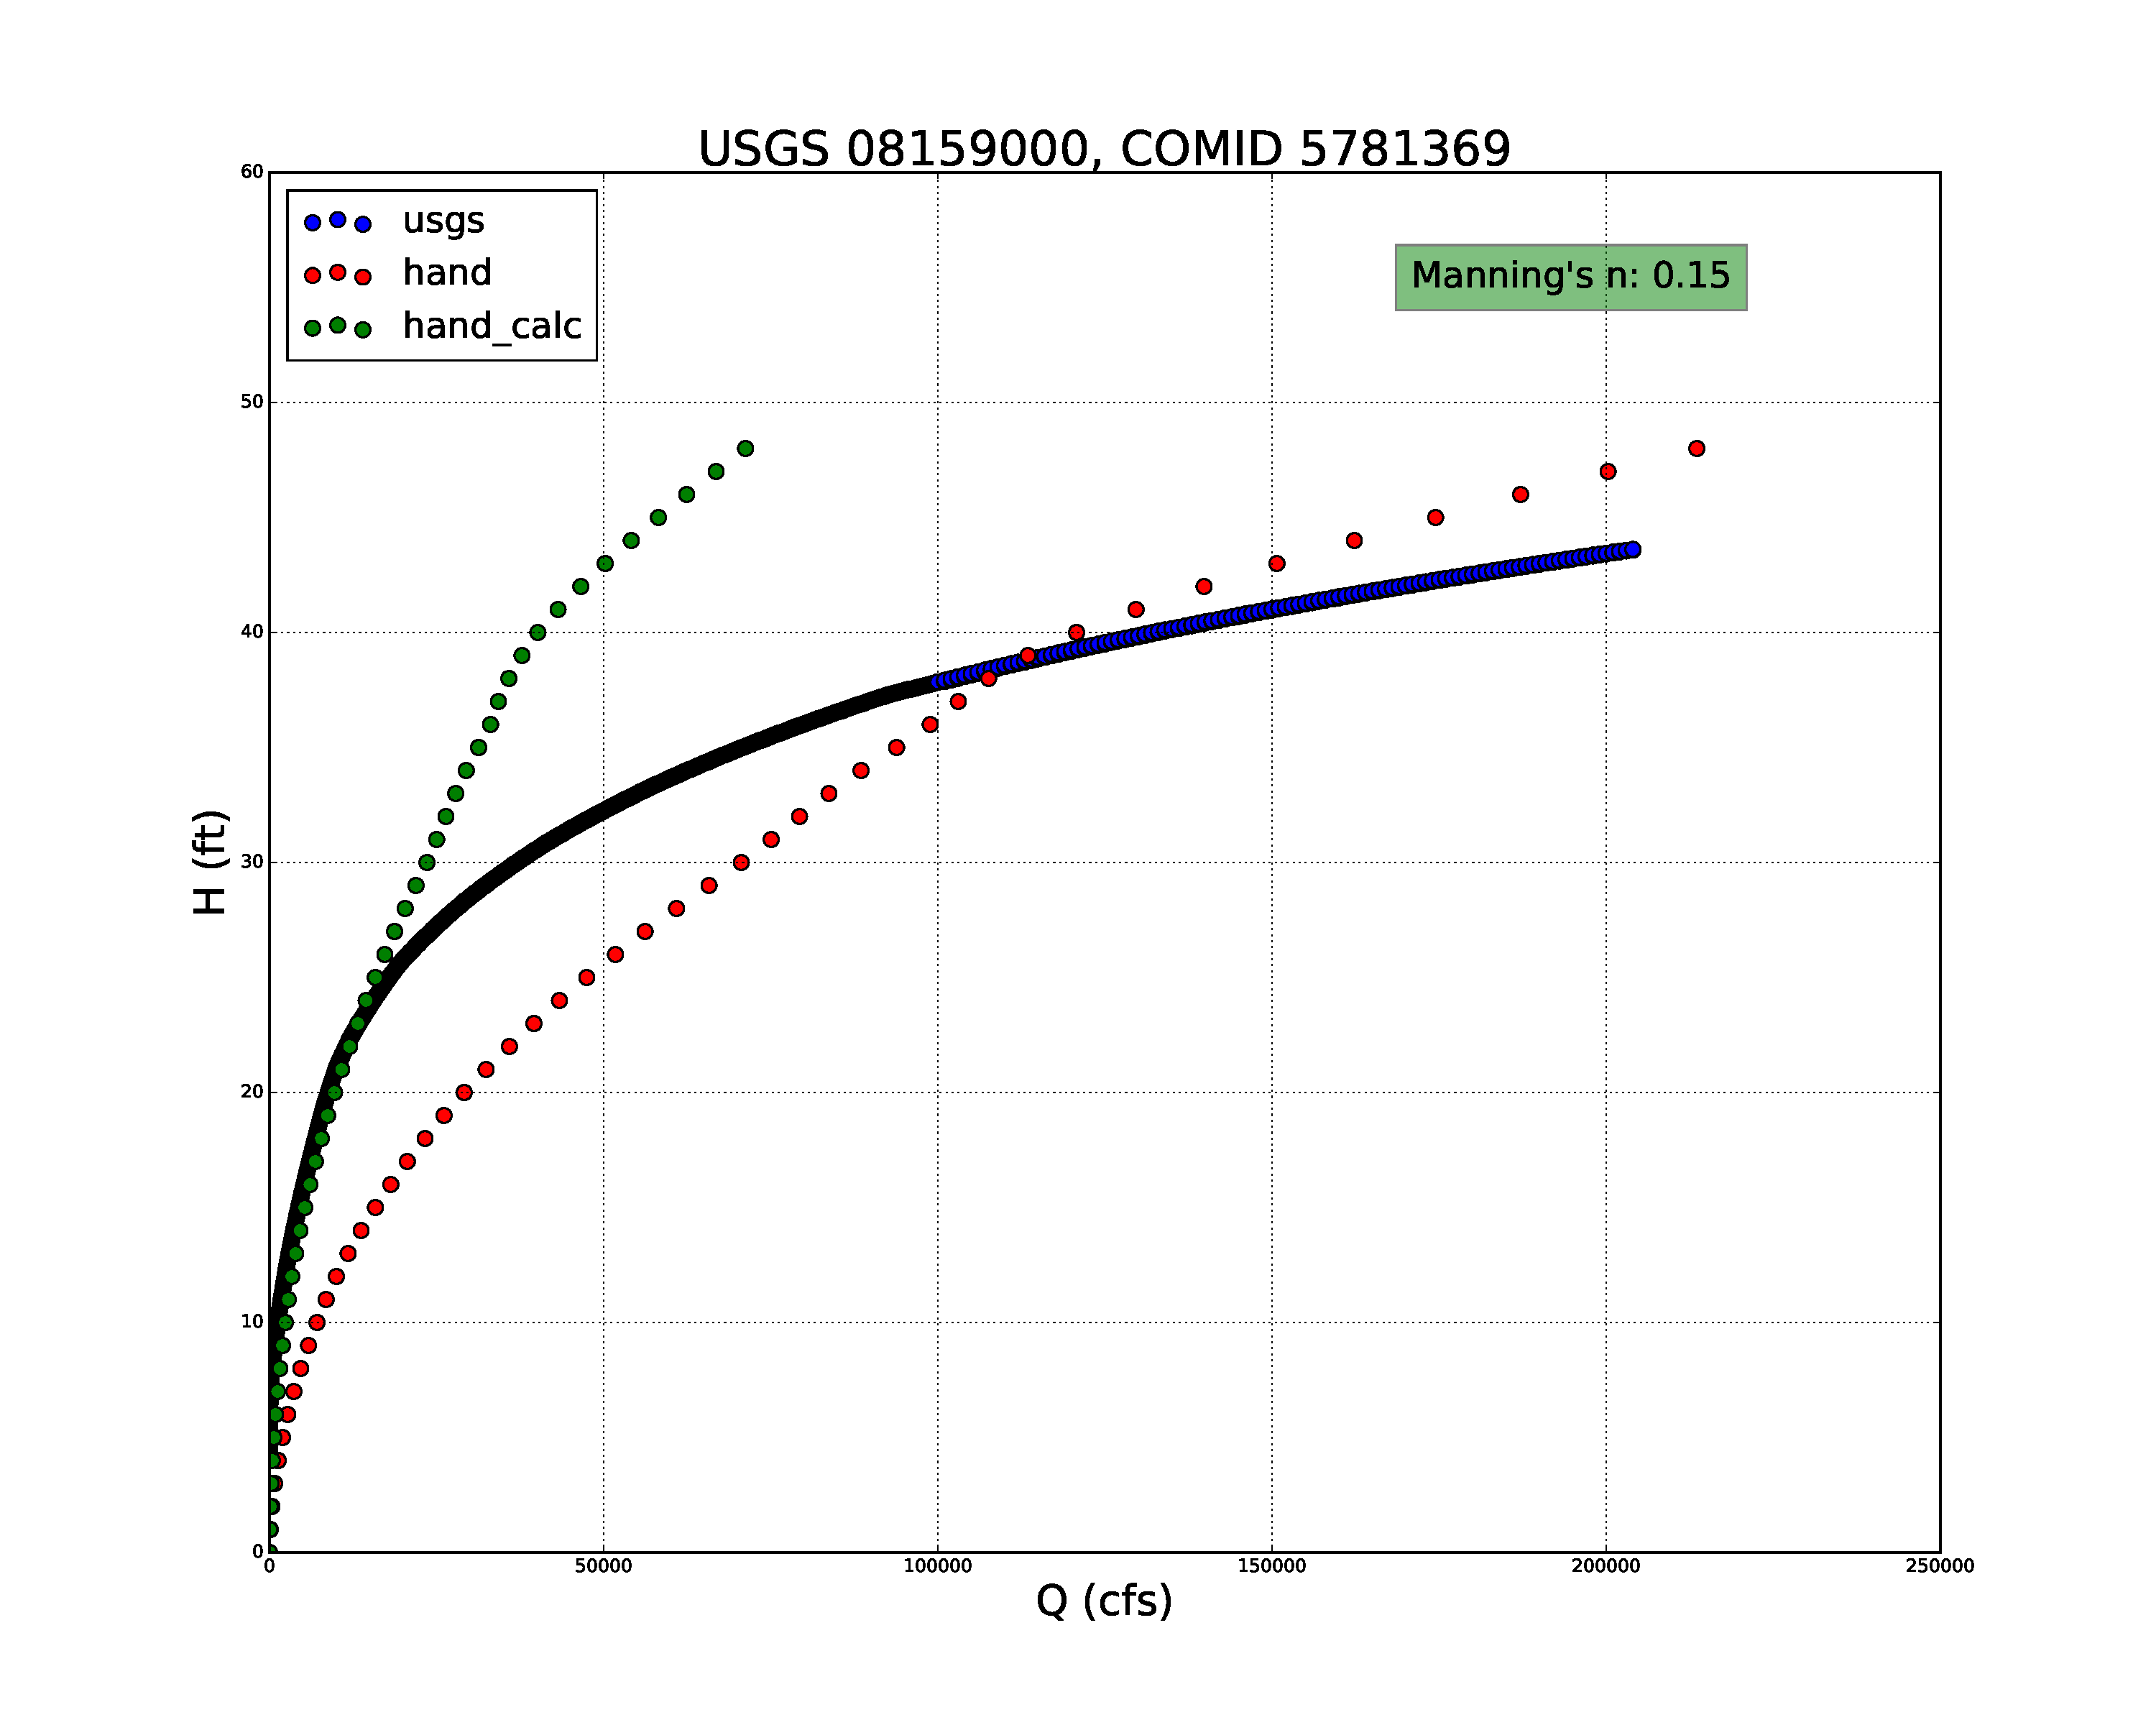
\includegraphics[width=\linewidth]{manualresults/rc_comid_5781369.pdf}
%   \caption{Manually-Adjusted Rating Curve}\label{fig:a}
% \end{subfigure}\hspace*{\fill}
% \begin{subfigure}{0.65\textwidth}
%   \centering
%   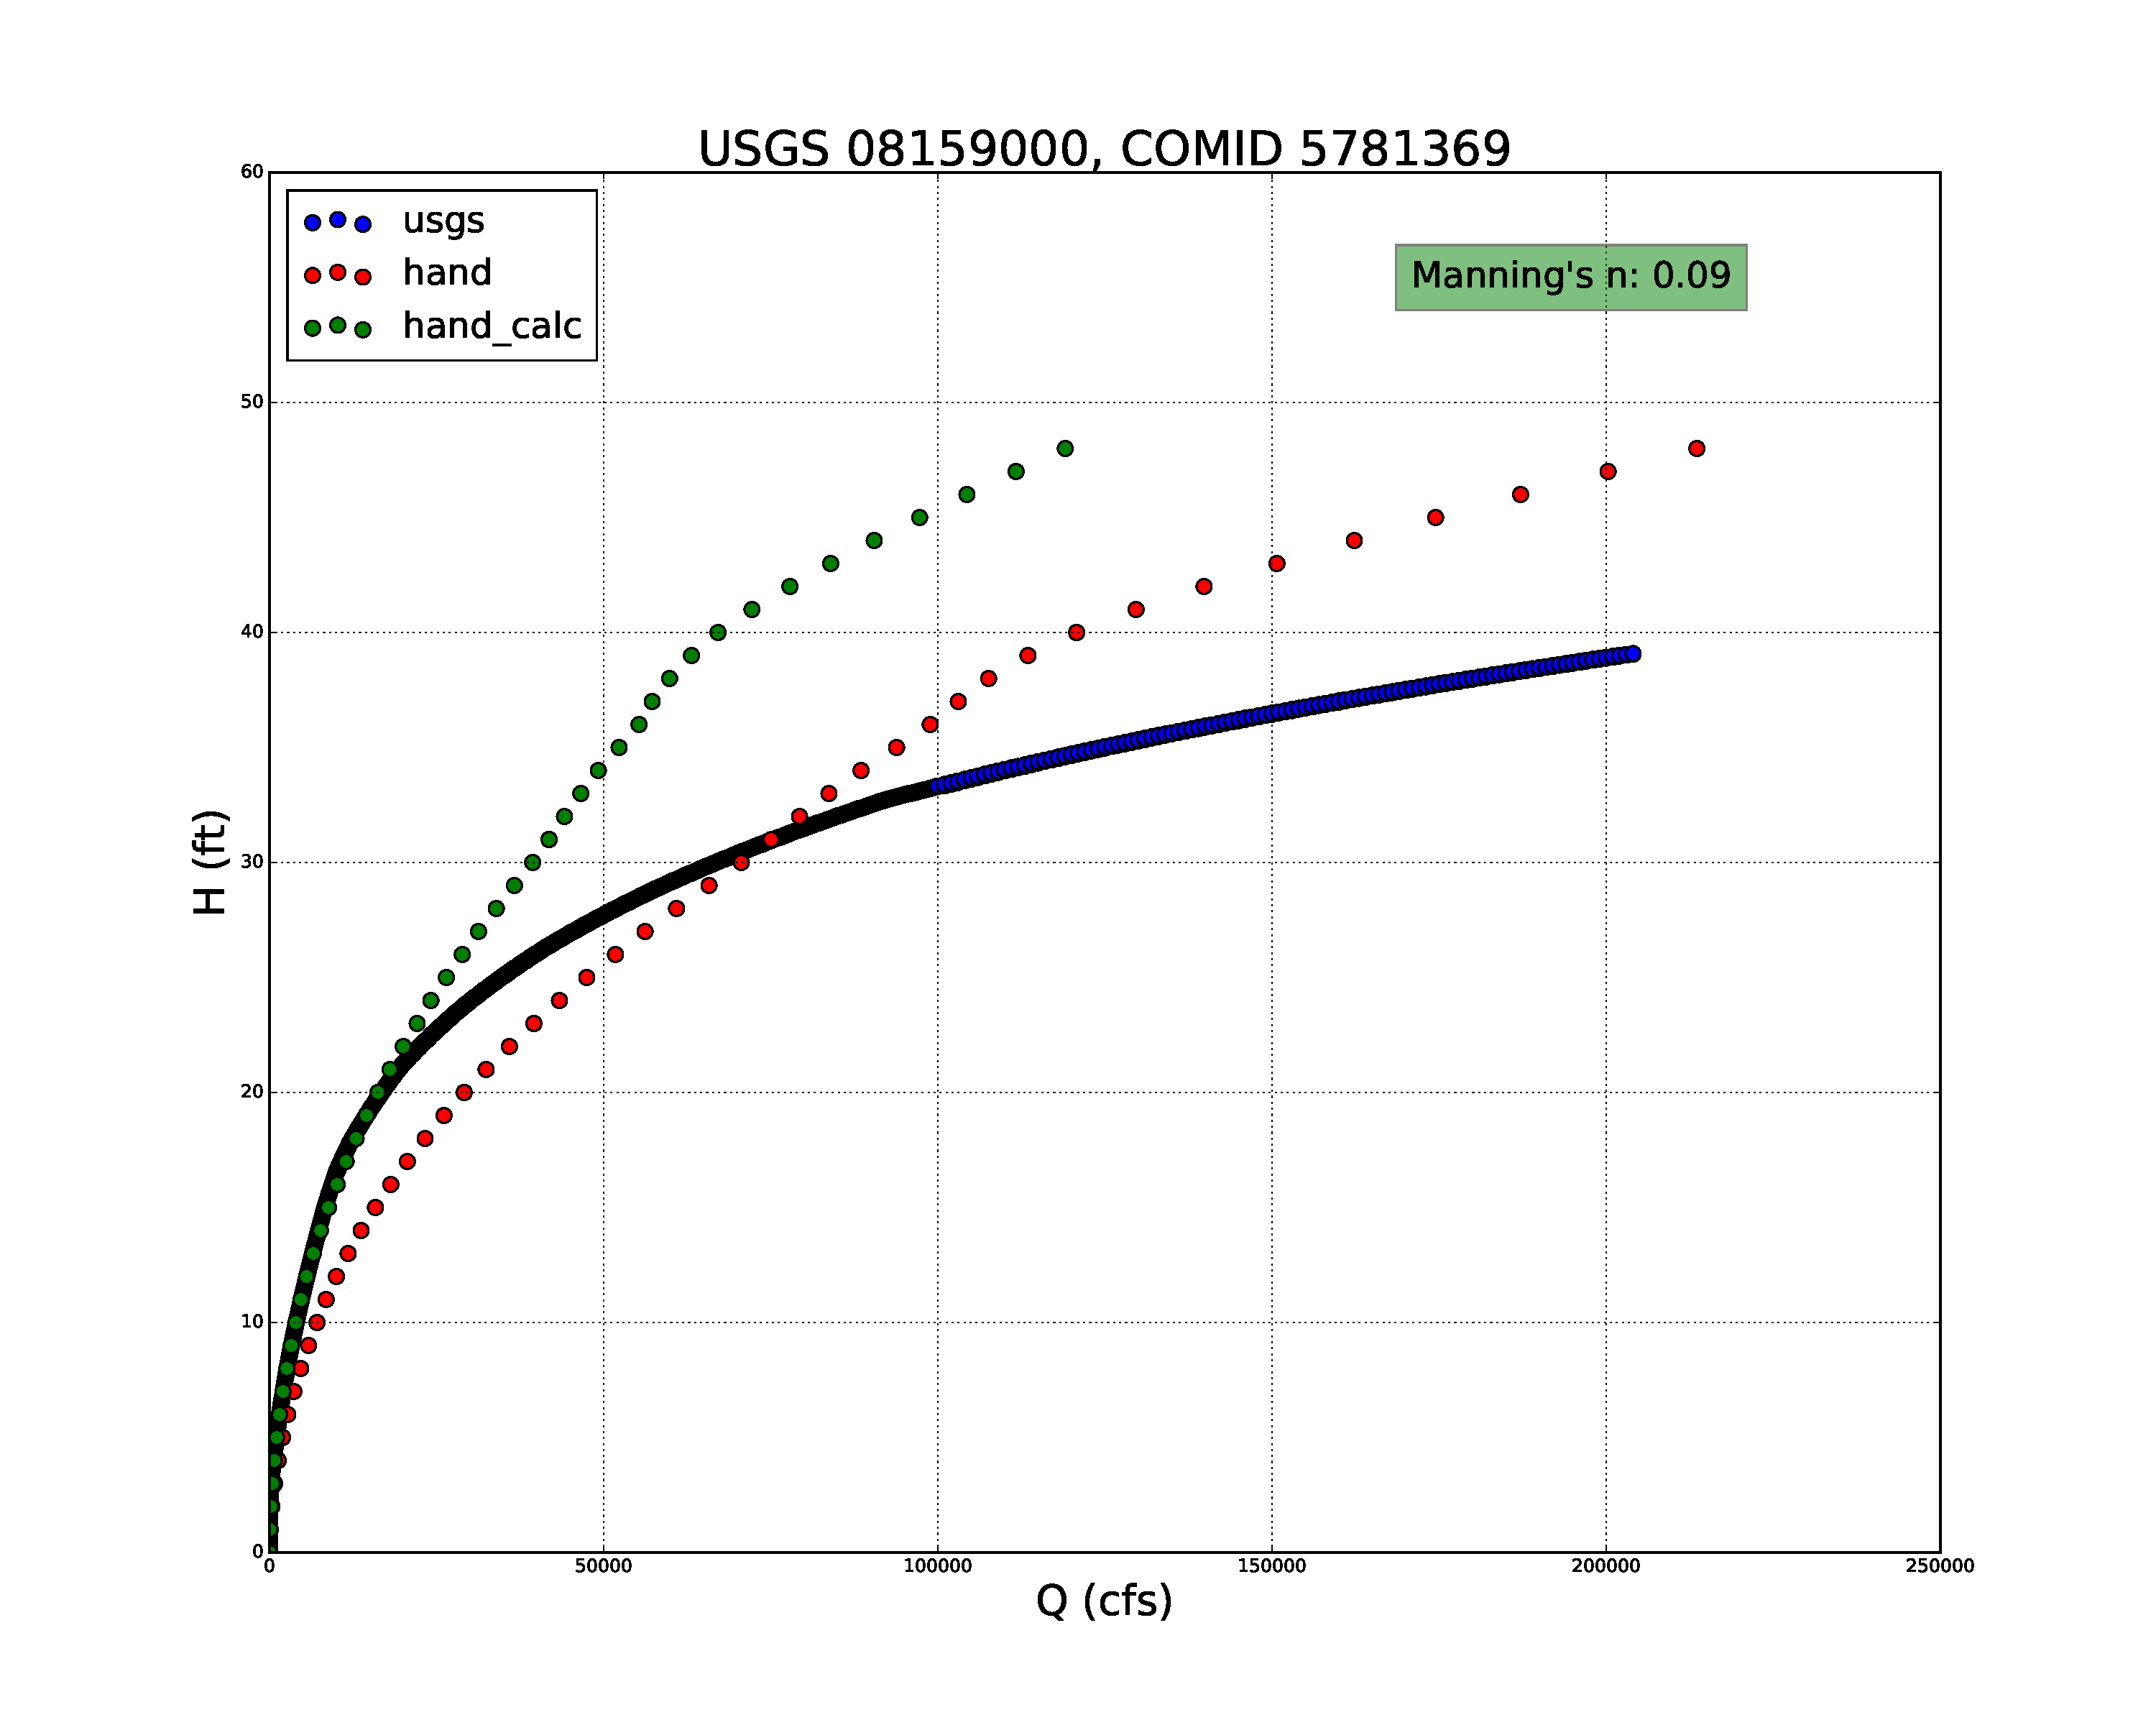
\includegraphics[width=\linewidth]{autoresults/rc_comid_5781369.pdf}
%   \caption{Automatically-Adjusted Rating Curve}\label{fig:b}
% \end{subfigure}\hspace*{\fill}
% }

% \caption{Manual vs. Automatic Adjustments for COMID 5781369 Rating Curve} \label{fig:3}
% \end{figure}

\begin{figure}[b!]
% \ContinuedFloat
\makebox[\linewidth][c]{
\begin{subfigure}{0.65\textwidth}
  \centering
  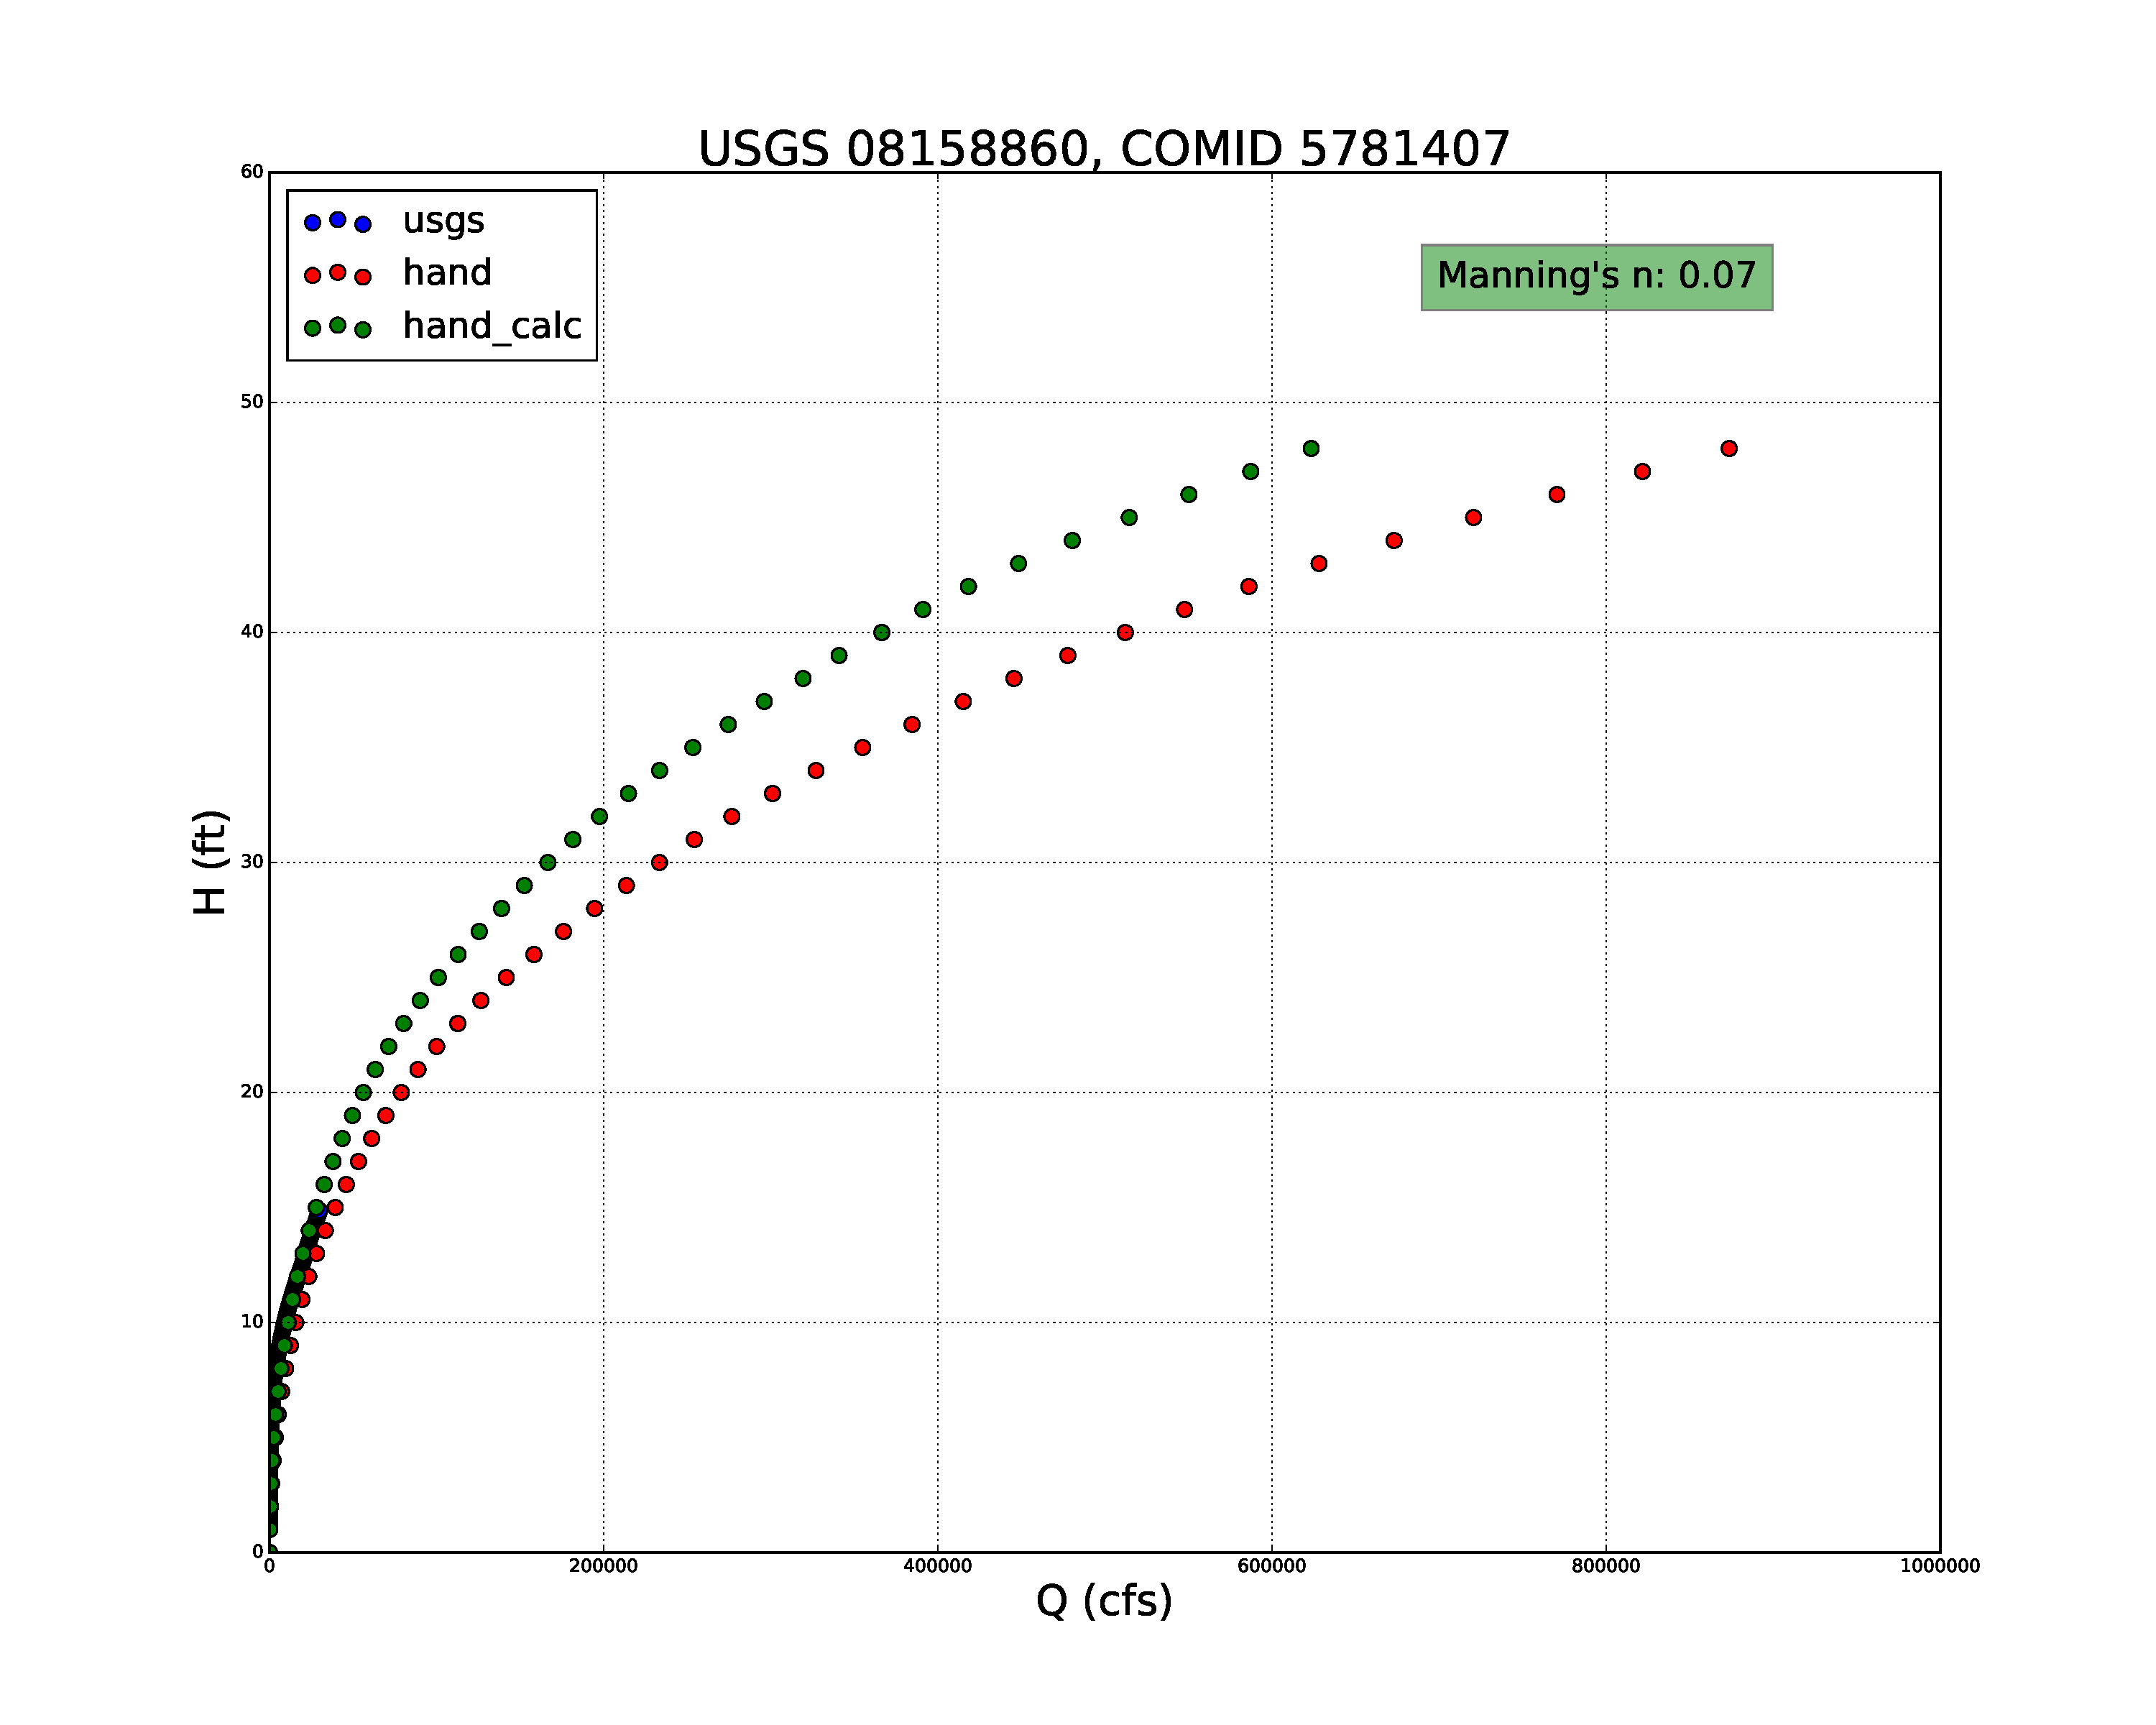
\includegraphics[width=\linewidth]{manualresults/rc_comid_5781407.pdf}
  \caption{Manually-Adjusted Rating Curve}\label{fig:a}
\end{subfigure}\hspace*{\fill}
\begin{subfigure}{0.65\textwidth}
  \centering
  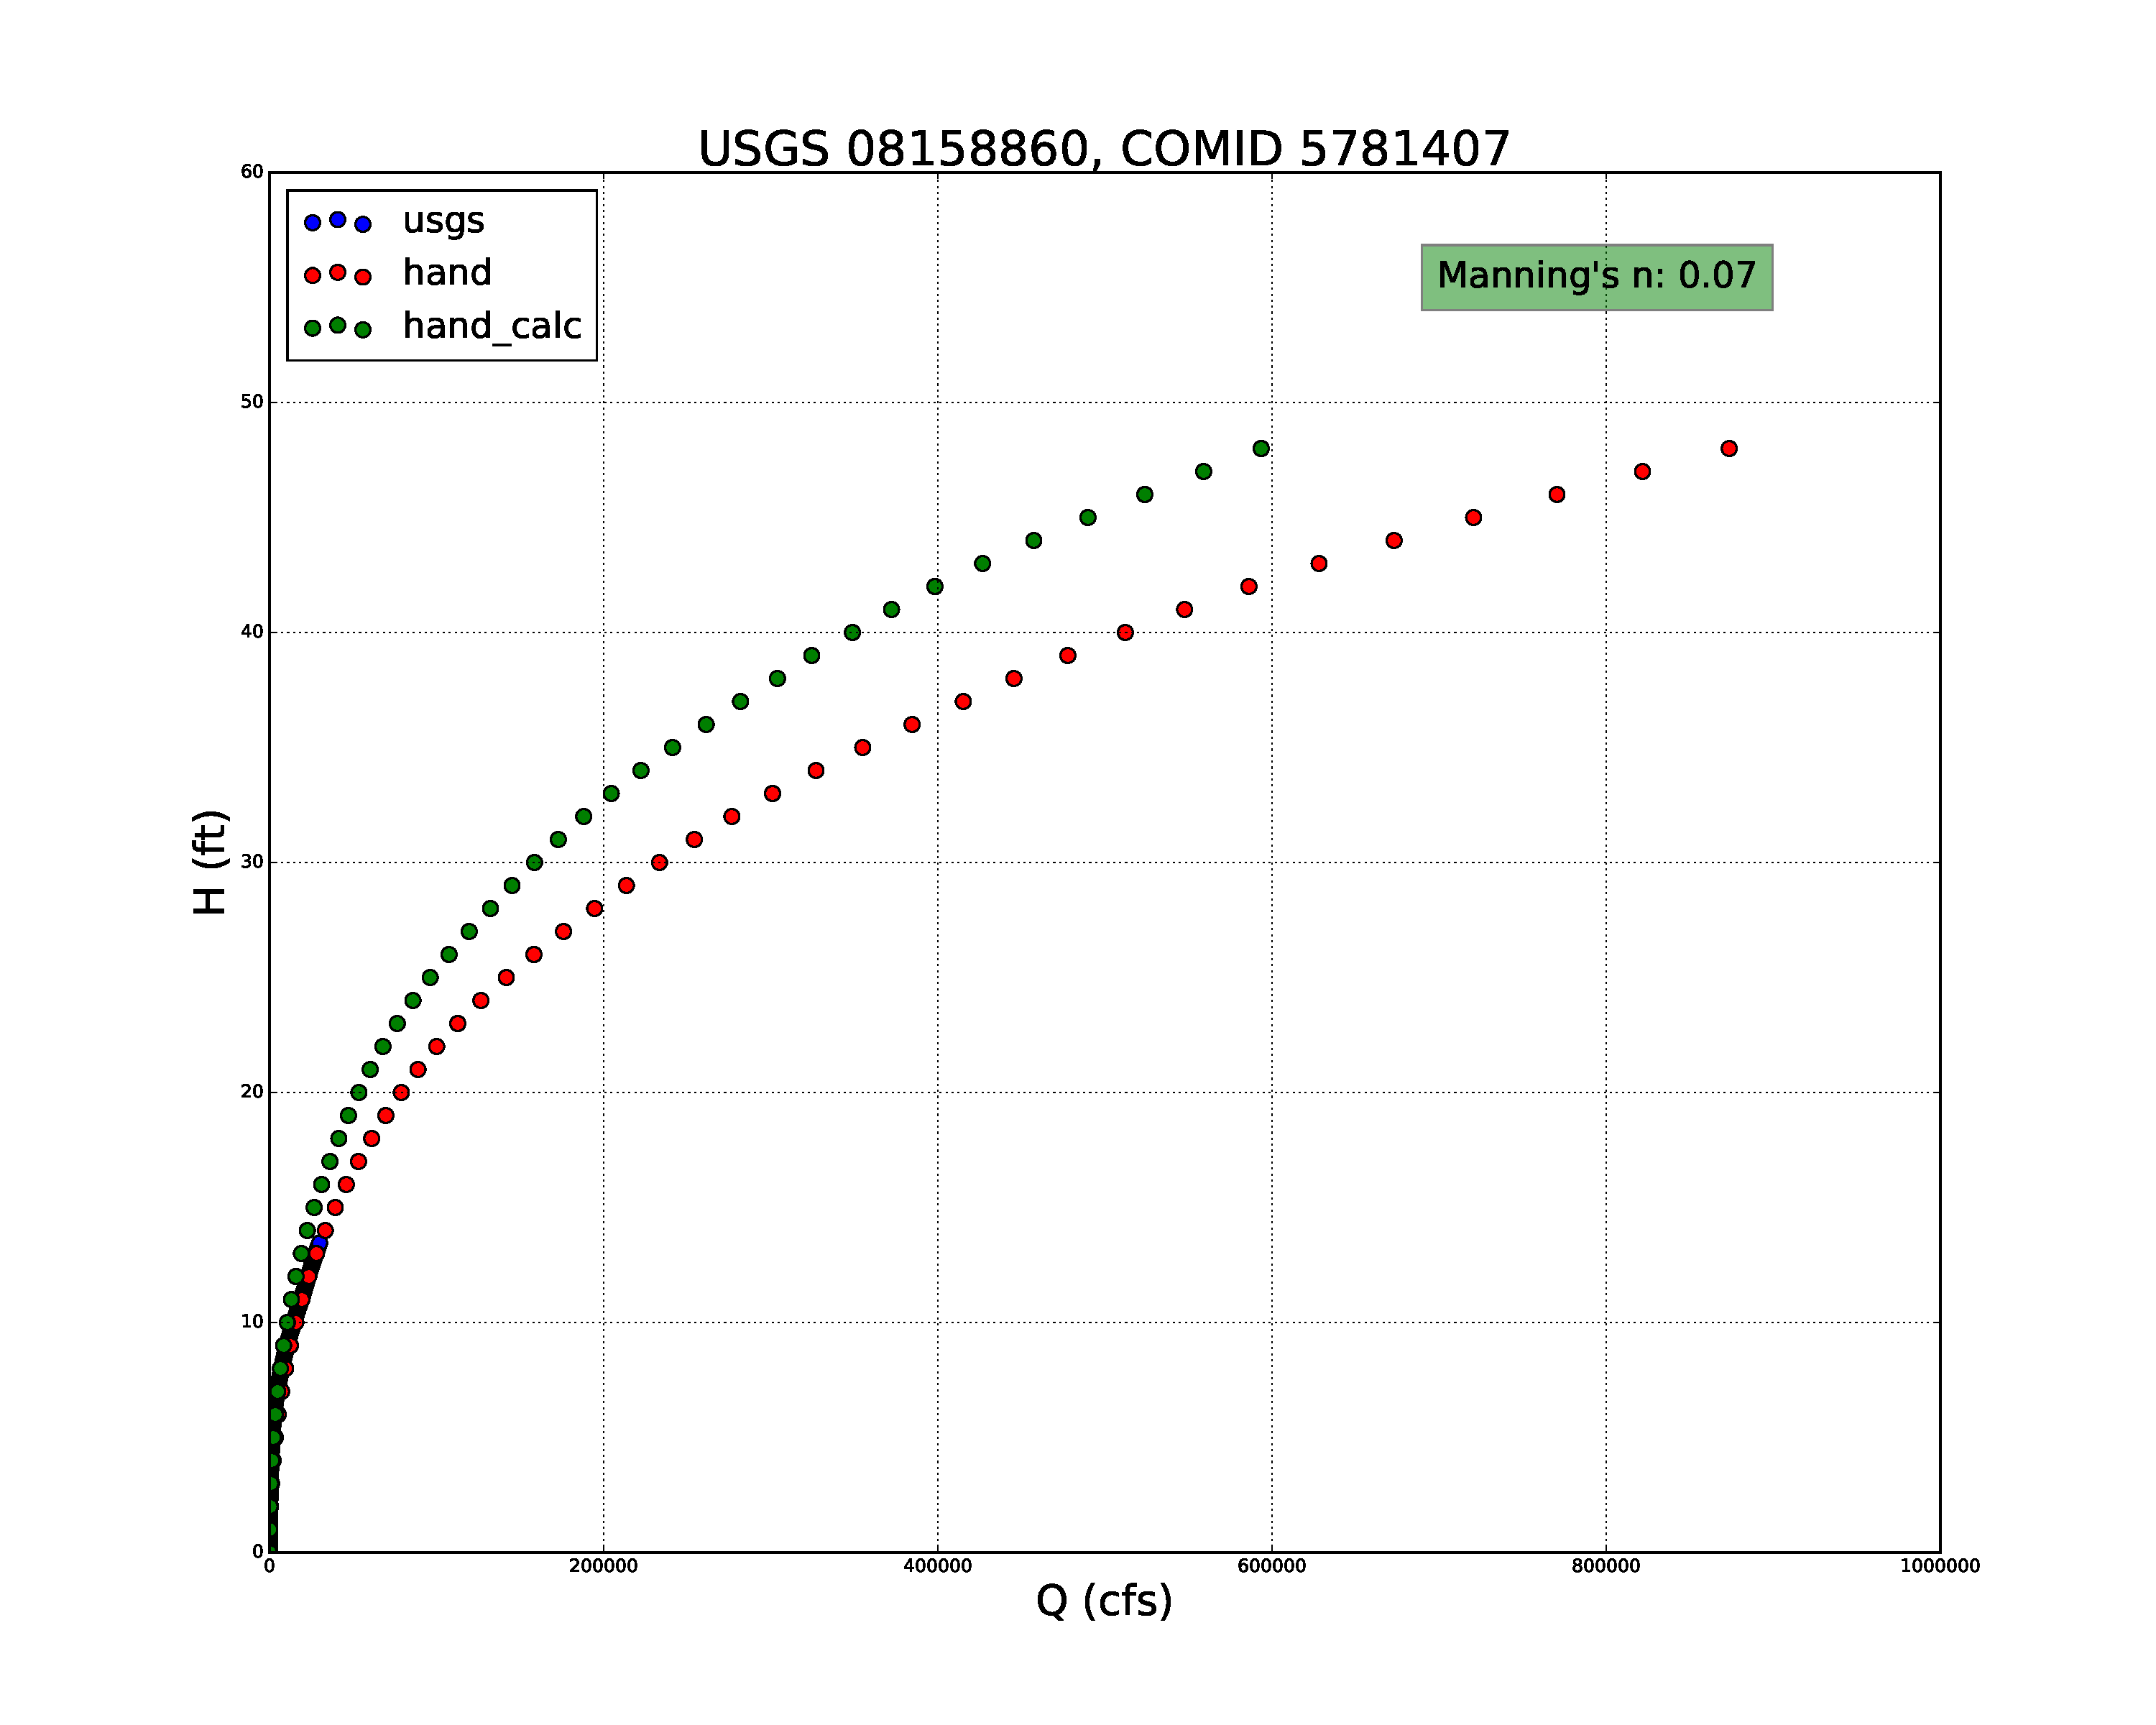
\includegraphics[width=\linewidth]{autoresults/rc_comid_5781407.pdf}
  \caption{Automatically-Adjusted Rating Curve}\label{fig:b}
\end{subfigure}\hspace*{\fill}
}

\caption{Manual vs. Automatic Adjustments for COMID 5781407 Rating Curve} \label{fig:4}
\end{figure}

\begin{figure}[b!]
% \ContinuedFloat
% \smallskip
\makebox[\linewidth][c]{
\begin{subfigure}{0.65\textwidth}
  \centering
  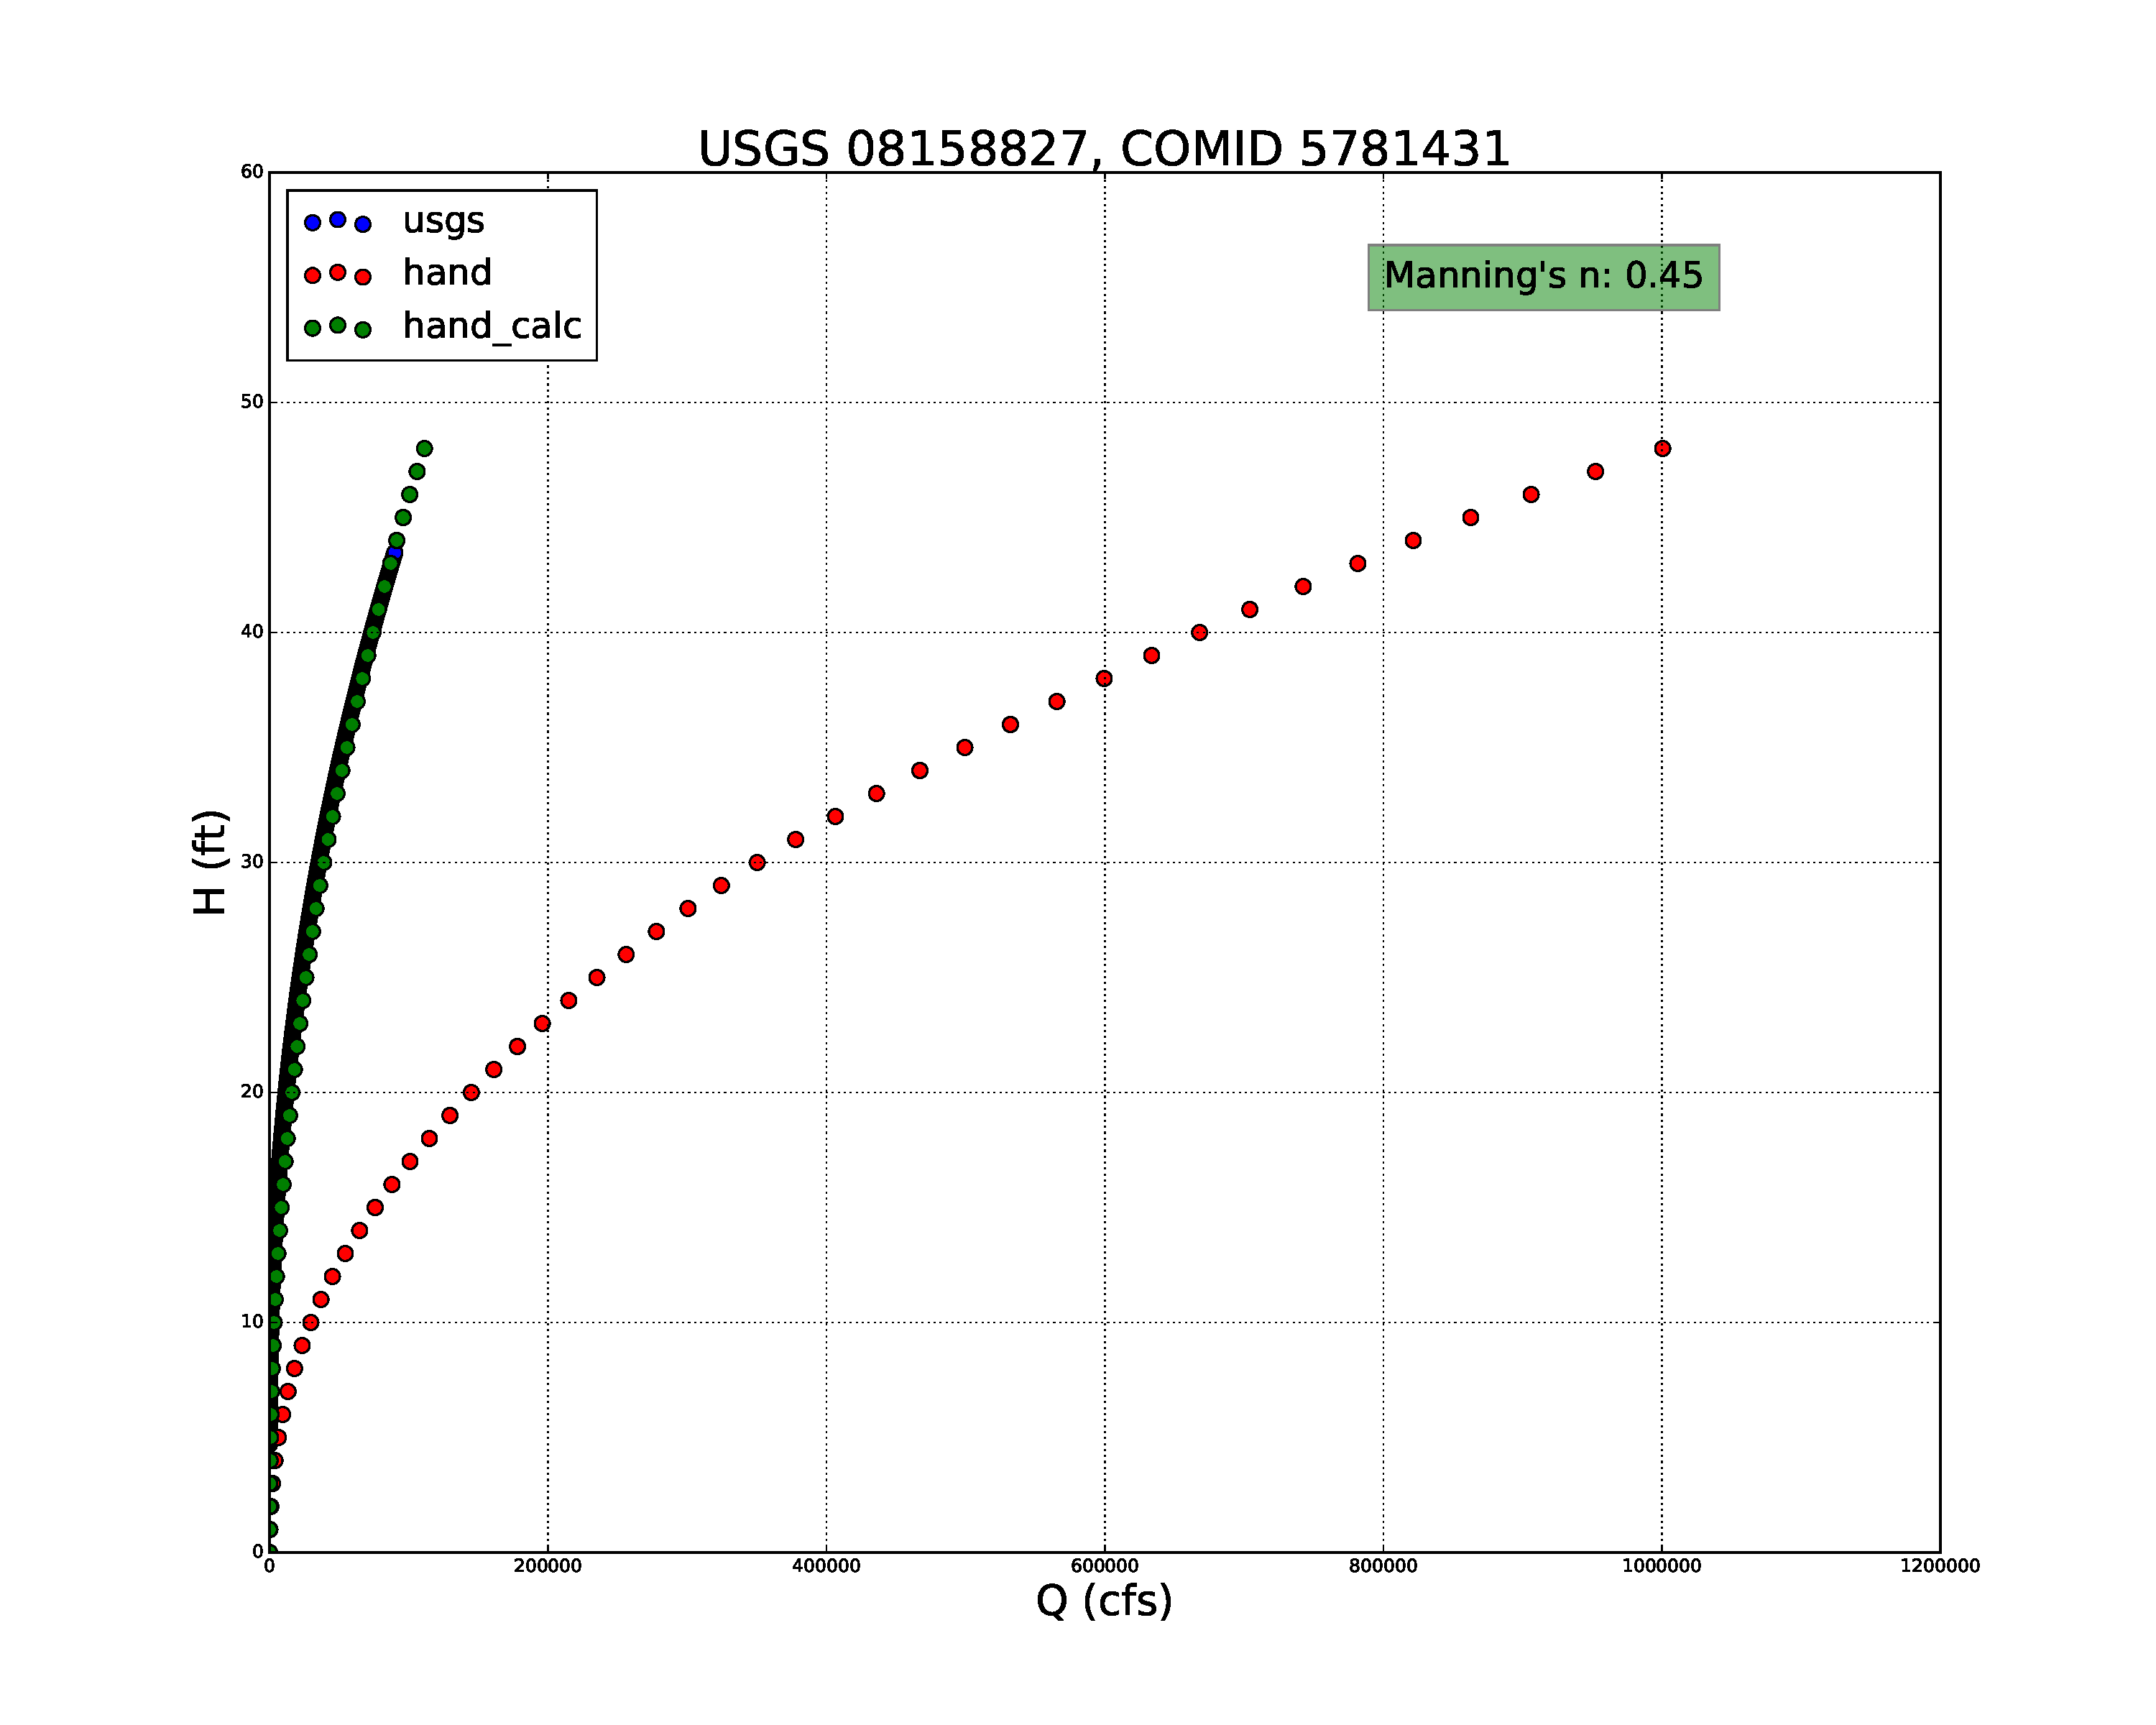
\includegraphics[width=\linewidth]{manualresults/rc_comid_5781431.pdf}
  \caption{Manually-Adjusted Rating Curve}\label{fig:a}
\end{subfigure}\hspace*{\fill}
\begin{subfigure}{0.65\textwidth}
  \centering
  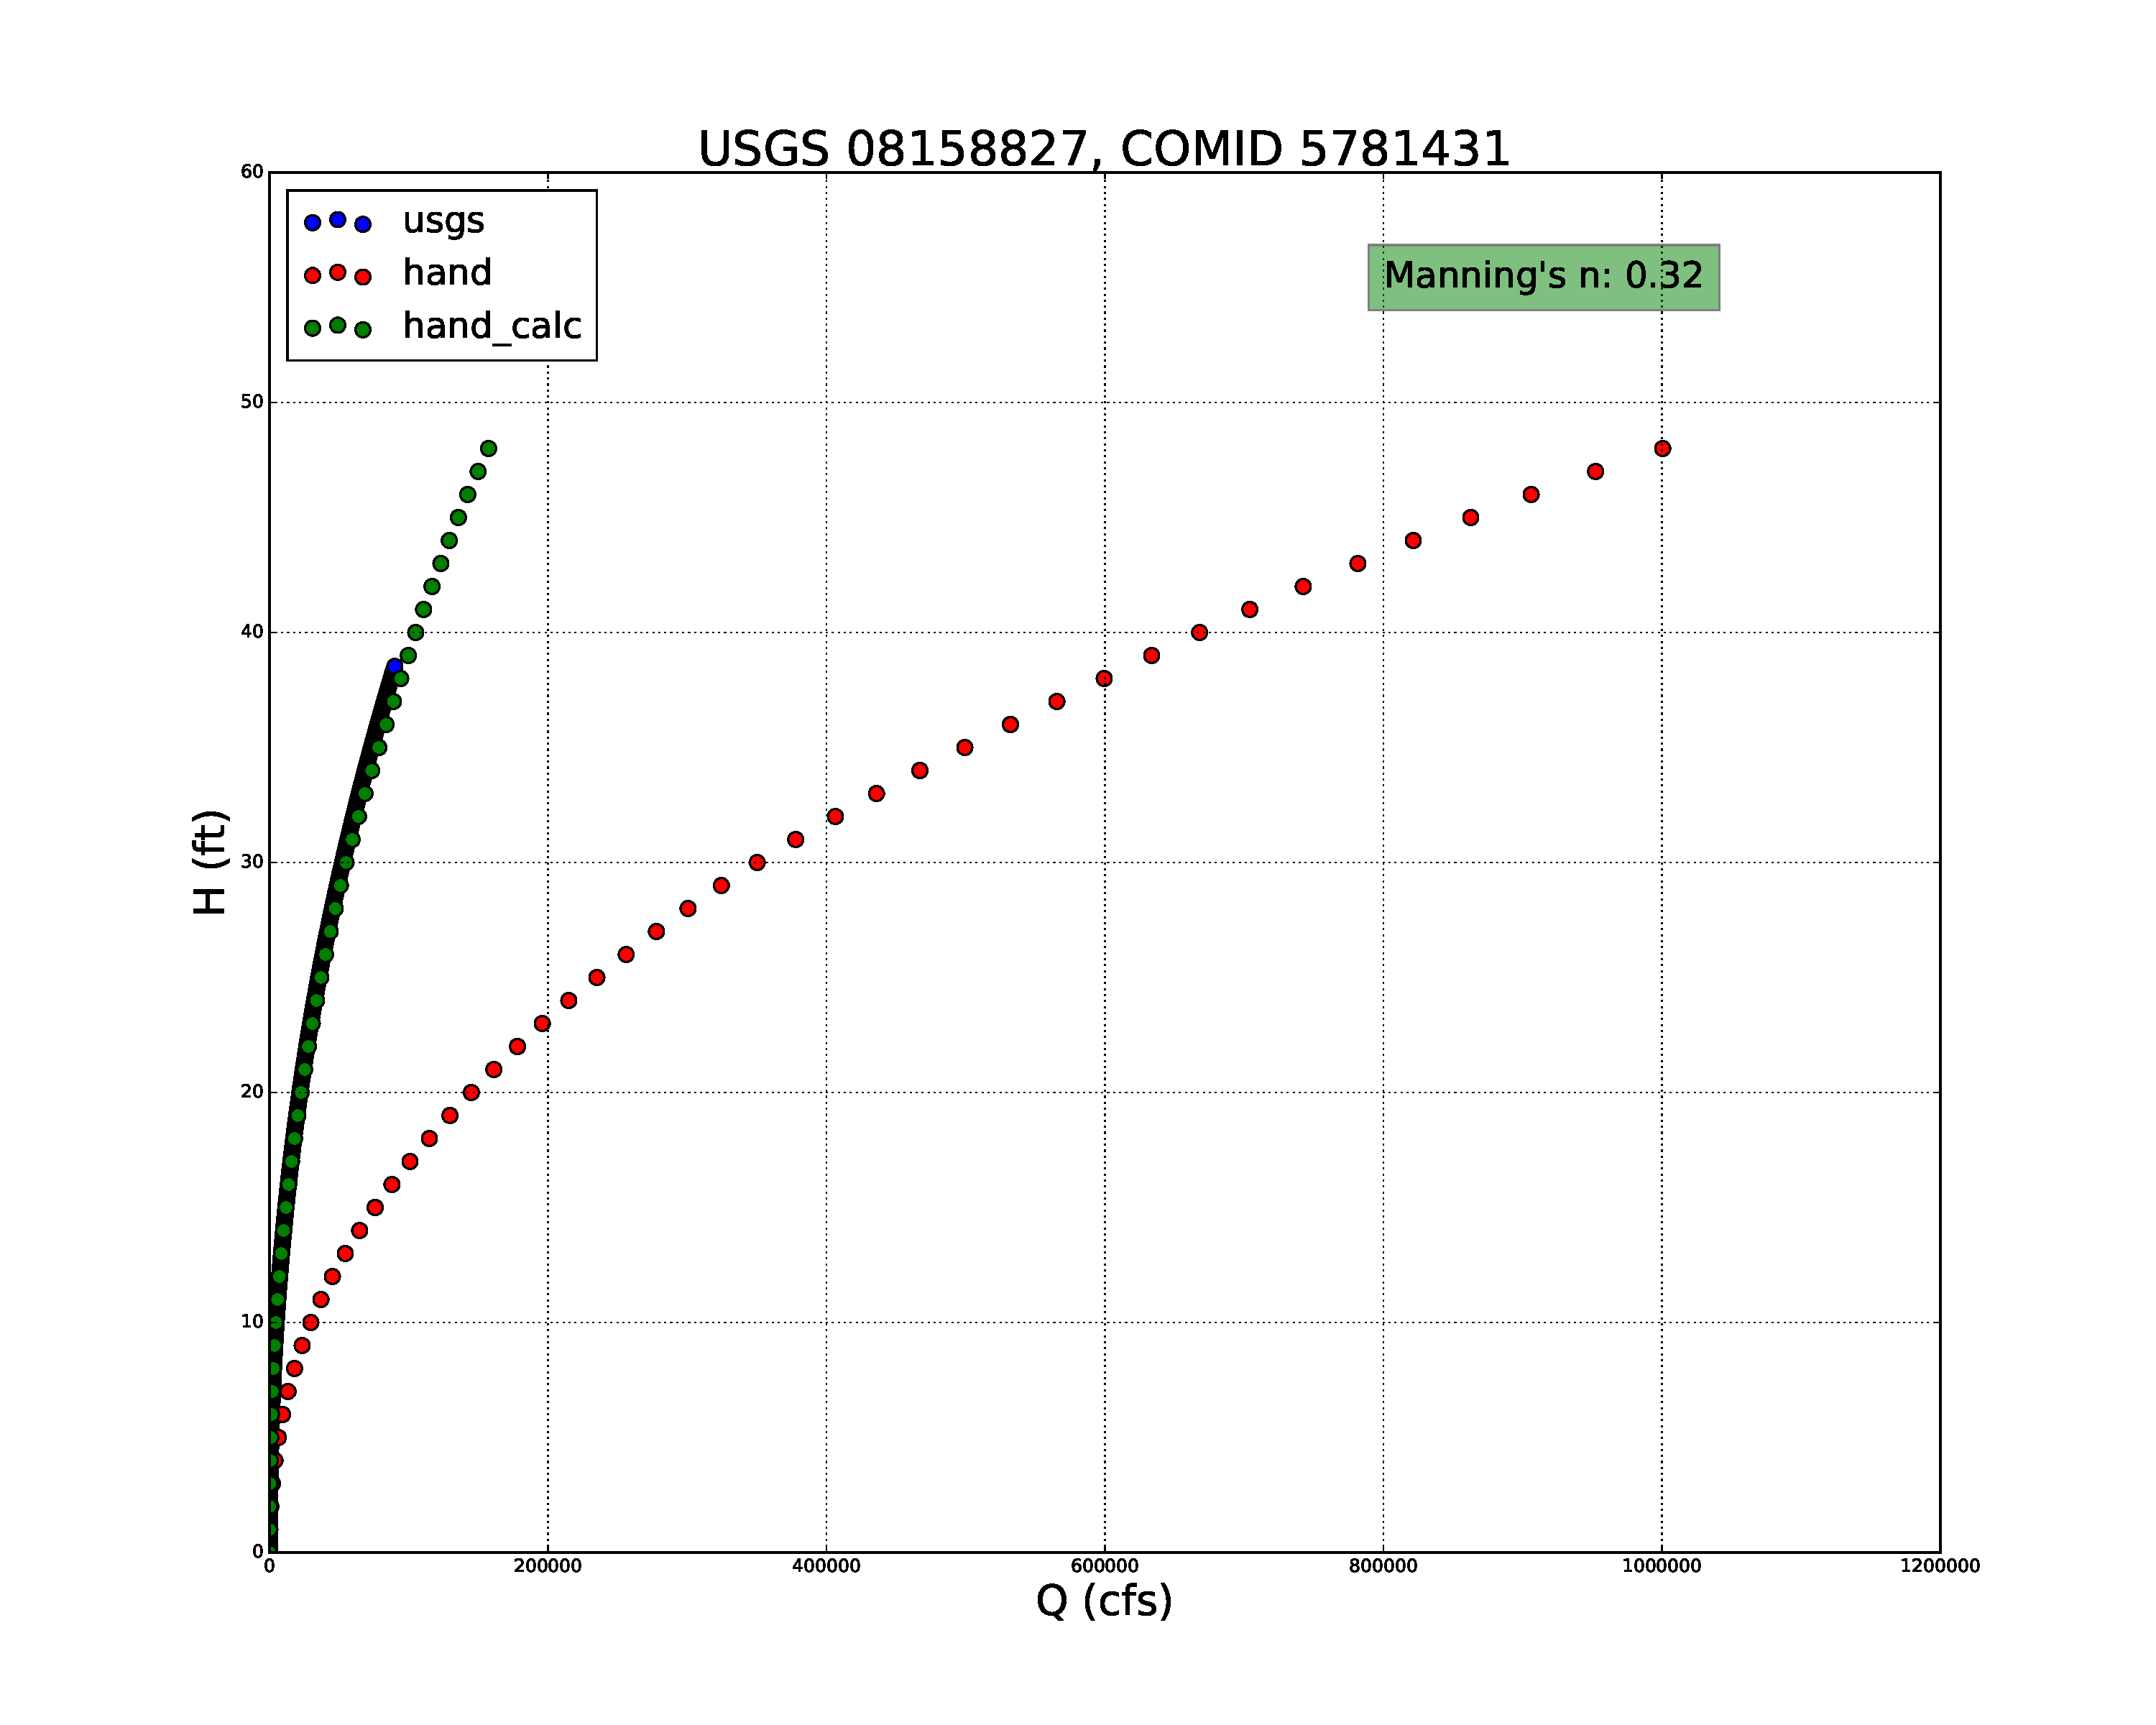
\includegraphics[width=\linewidth]{autoresults/rc_comid_5781431.pdf}
  \caption{Audomatically-Adjusted Rating Curve}\label{fig:b}
\end{subfigure}\hspace*{\fill}
}

\caption{Manual vs. Automatic Adjustments for COMID 5781431 Rating Curve} \label{fig:5}
\end{figure}

\clearpage

As stated previously, the intent of this research is to programmatically fit a HAND rating curve to its corresponding USGS rating curve. That said, manipulation of manning's $n$ is not strictly acceptable, seeing as it is a physical parameter ideally representative of the stream reach in question (see figure 1 below). Changes to manning's $n$ are effectively a claim that physical streambed material is changing, which is unreasonable. Instead, this project has changed to focus on understanding the statistical differences between "theoretical" hydrologic properties (specifically wetted area, hydraulic radius, and slope) and their "actual" counterparts, which will likely be retrieved from HEC-RAS models with detailed cross-section descriptions.

\begin{figure}[b!]
\centering
\includegraphics[keepaspectratio, width=\textwidth]{n_values.pdf}
\caption{Acceptable Manning's $n$ values, retrieved from: \url{http://www.shippensburgtownship.com/2010-01/media/development/Table\%20B-4.pdf}} \label{fig:1}
\end{figure}

After the data was collected, a preliminary assessment was conducted in which the ``correct'' manning's $n$ for each of eight stream reaches within the Onion Creek watershed were manually determined. Figures 1a through 1h (see pages 3 and 4) show both the HAND rating curves (red), the USGS rating curves (blue), and the HAND rating curve after it has been manually fitted to the USGS rating curve (green); the manning's $n$ value displayed in the upper right-hand corner of each image is the roughness that was used for the fit. \\

The first thing that is evident is that the ``correct'' manning's $n$ values are quite high. As seen in the following url: \url{http://www.fsl.orst.edu/geowater/FX3/help/8_Hydraulic_Reference/Mannings_n_Tables.htm}, manning's $n$ is generally between 0.02 and 0.07, with values rarely getting above 0.2. As such, I will need to spend some time reviewing the Python script I am using (Listing 1) to be certain that my mathematical approach and units are correct. Once I am certain that the mathematics is correct, I will proceed to automate the curve fitting. 

\noindent
Regarding the automation of the curve fitting, there are two main steps: 

\begin{enumerate}
  \item Adjust HAND rating curve to fit USGS rating curve along the y-axis (Height, ft) to correct for the USGS accepted bank bottom. I am still devising the solution to this problem, but -- after taking into account the vertical ``shift'' -- I believe I will need to find the highest depth associated with a discharge of zero (USGS rating curves often have many depths with Q = 0, including depths up to multiple feet high) and then set that height as a ``true'' zero. Once this zero is obtained, I will need to correct the HAND rating curve heights to shift them appropriately. 
  \vspace{1ex}
  \item Fit each vertically-adjusted HAND rating curve to the USGS rating curve by taking each HAND height and it's associated hydraulic parameters, and looking up the discharge associated with that height in the USGS rating curve table; with all these data points, manning's $n$ can easily be computed and averaged over all heights for each stream reach. This idea should work fine, but I am skeptical that the results will be beneficial: by relying on the USGS rating curves to compute the HAND rating curves, I can not see a clear path forward for generalizing the HAND rating curve computation for reaches without USGS rating curves. As such, I think a statistical approach would be best for the long-term. I'm not entirely sure how this approach may work, but I would suspect there are ways to statistically fit the HAND rating curves to the USGS rating curves (by minimizing the difference between discharge values at the same height, perhaps using an ANOVA or Kruskal-Wallis test and accepting the fit once the null hypothesis is no longer rejected). I am also anticipating that we will learn ways for statistically correlating datasets, such that I may correlate manning's $n$ with the National Land Cover Dataset I mentioned in the first portion of this assignment. 
\end{enumerate}

Both these steps are starting to come together, but this is still a work in progress and as such any advice would be very welcome. The intent at this point is to proceed with steps 1 and 2 until Onion Creek is working appropriately. Once this is done, I will try to expand my code to function on all of the stream reaches in Texas that have USGS gage locations. To do this, I will test over some fraction of the stream reaches (ie. 90\%), use the results to inform some sort of machine-learning algorithm that I hope to implement, and finally verify and/or validate the functionality on the remaining smaller fraction (ie. 10\%) of the stream reaches in Texas. This would make room for a further statistical analysis of the correctness of my algorithm, and once that analysis passes in a statistically-significant manner, I can safely proceed to automate my problem for all of Texas (including all stream reaches that do not contain USGS rating curves for potential validation). \\

\clearpage

\lstinputlisting[language=Python, firstline=10, lastline=93, caption={Class CompareRC defined in ratingcurves-onionck-clean.py module to quickly collect, extract, calculate, and display the USGS/HAND rating curves shown in Figure 1.}]{../../../../research/ratingcurves/ratingcurves-onionck.py}

\end{document}